\section{STL-Datenstrukturen}

\subsection{Überblick}

\begin{frame}[fragile]{Standard Template Library}
	Aufbau: building blocks
	
	\vspace{1em}
	
	\begin{itemize}
		\item containers, adaptors
		\item streams
		\item algorithms
		\item functional programming
		\item helpers (e.g. \verb|reference_wrapper|)
		\item metaprogramming support
	\end{itemize}
\end{frame}

\begin{frame}[fragile]{Standard Template Library}
	Alexander Stepanov, Mitbegründer des generic programming und der STL:
	{\tiny aus: Forward to \enquote{STL Tutorial and Reference Guide, Second Edition} }
	
	\begin{block}{Fundamental ideas behind STL}
		\begin{itemize}
			\item Generic programming
			\item Abstractness without loss of efficiency
			\item Von Neumann computational model (pointers)
			\item Value semantics (whole-part ownership)
		\end{itemize}
	\end{block}
	
	\pause
	
	\vspace{2em}
	\enquote{Fun fact} \emph{;)}\\
	STL $\subset$ Standard-Bibliothek
\end{frame}


\subsection{sequence containers}

\begin{frame}[fragile]{Überblick}
	Die STL stellt für die geordnete Speicherung von \enquote{Dingen} drei Containertypen bereit:
	\begin{itemize}
		\item \verb|vector|
		\item \verb|list|
		\item \verb|deque|
	\end{itemize}
	
	\pause
	
	Außerdem gibt es noch drei Adapter-Typen, die auf Basis dieser Container arbeiten:
	\begin{itemize}
		\item \verb|queue|
		\item \verb|priority_queue|
		\item \verb|stack|
	\end{itemize}
	
	\pause
	
	Diese werden in einem der nächsten Workshops besprochen.
\end{frame}

\begin{frame}[fragile]{Gemeinsame Eigenschaften/Funktionalität}
	\begin{itemize}
		\item Speichern Sequenzen von \enquote{Dinge}
		\begin{itemize}
			\item In der vorgegebenen Reihenfolge (Überraschung!)
			\pause
			\item Dynamisch, sie passen ihre Größe den Anforderungen an
		\end{itemize}
	\end{itemize}
	
	\pause
	
	Funktionsumfang:
	\begin{itemize}
		\item Zugriff über Iteratoren (mehr dazu später)
		\begin{itemize}
			\item Sowohl vorwärts als auch rückwärts
			\item Generell je Inkrement in $\mathcal{O}(1)$
		\end{itemize}
		\pause
		\item Elementzählung in $\mathcal{O}(1)$
		\pause
		\item Elementzugriff
		\begin{itemize}
			\item Anfang und Ende in $\mathcal{O}(1)$
			\item \verb|vector| und \verb|deque| auch Wahlfrei (in $\mathcal{O}(1)$)
		\end{itemize}
		\pause
		\item Modifikation: Einfügen, löschen und leeren
	\end{itemize}
\end{frame}

\begin{frame}[fragile]{Container: \texttt{vector}}
	\begin{block}{Abbildung: Struktur}
		\begin{center}
			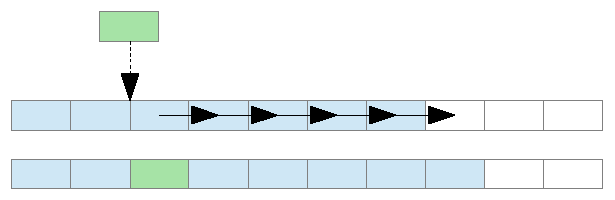
\includegraphics[width=0.6\linewidth]{images/vector.pdf}
		\end{center}
	\end{block}

	\begin{itemize}
		\item Array-basiert
		\pause
		\begin{itemize}
			\item[+] Cache-effizient
			\item[+] (Direkt-)Zugriffe sehr schnell möglich: $\mathcal{O}(1)$
			\pause
			\item Wachstum erfordert Kopiervorgänge!
			\item[-] Einfügen/Entfernen ist teuer: $\mathcal{O}(n)$ (!)
			\begin{itemize}
				\item Ausnahme: Am Ende des \verb|vector|s (mit \verb|push_back|, \verb|pop_back|): $\mathcal{O}(1)$
			\end{itemize}
		\end{itemize}
		\pause
		\item Vor allem geeignet für Aufgaben mit wahlfreiem Zugriff und wenigen Änderungsoperationen die nicht am Ende stattfinden.
	\end{itemize}
\end{frame}
	
\begin{frame}[fragile]{Container: \texttt{list}}
	\begin{block}{Abbildung: Struktur}
		\begin{center}
			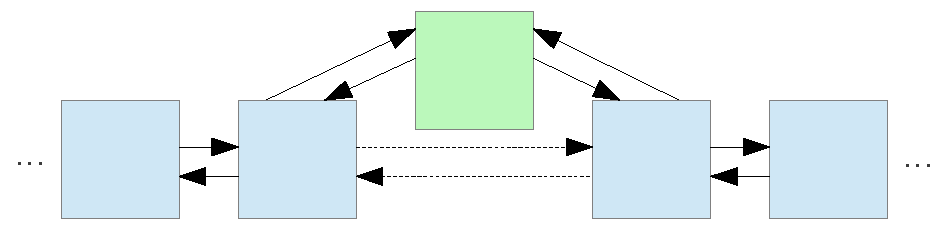
\includegraphics[width=0.6\linewidth]{images/list.pdf}
		\end{center}
	\end{block}

	\begin{itemize}
		\item Zugrundeliegende Datenstruktur: Doppelt verkettete Liste
		\pause
		\begin{itemize}
			\item[-] Schlechte Cache-Effizienz (nichtkontinuierliche Speicherbelegung)
			\item[-] Kein Direktzugriff! Über Iteration in $\mathcal{O}(n)$ (!)
			\pause
			\item[+] Einfügen/Entfernen ist (bei gegebener Position) sehr schnell: $\mathcal{O}(1)$
			\item[+] Verschieben von Elementen in eine andere \verb|list| ist (in zwei Fällen) sehr schnell: \verb|splice| in $\mathcal{O}(1)$
		\end{itemize}
		\pause
		\item Vor allem geeignet für Algorithmen mit einer großen Anzahl nichttrivialer Listenmodifikationen, solange kein wahlfreier Zugriff erforderlich ist.
	\end{itemize}
\end{frame}

\begin{frame}[fragile]{Container: \texttt{deque}}
	\begin{block}{Abbildung: Struktur}
		\begin{center}
			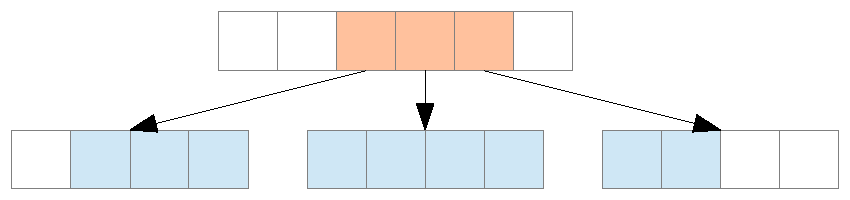
\includegraphics[width=0.6\linewidth]{images/deque.pdf}
		\end{center}
	\end{block}
	
	\begin{itemize}
		\item Datenstruktur: Array-basiert ähnlich wie \verb|vector|, aber in kleine Blöcke unterteilt
		\pause
		\begin{itemize}
			\item[+] Cache-Effizienz: Zusammenhängende Blöcke $\rightarrow$ vermutlich gut
			\item[+] Direktzugriff: $\mathcal{O}(1)$
			\pause
			\item Wieder: Wachstum erfordert Kopieroperationen
			\item[-] Beliebiges Einfügen/Entfernen: $\mathcal{O}(n)$ (wie bei \verb|vector|)
			\begin{itemize}
				\item Ausnahme: An Anfang oder Ende der \verb|deque| (\verb|push|/\verb|pop_front|/\verb|back|): $\mathcal{O}(1)$
			\end{itemize}
		\end{itemize}
		\pause
		\item \verb|deque| ist etwas flexibler als \verb|vector|, hat aber auch einen größeren Verwaltungsoverhead. (Konstante Faktoren!)
	\end{itemize}
\end{frame}

\begin{frame}{Codebeispiel}
	\lstinputlisting[basicstyle=\scriptsize]{cpp-code/sequence-usage.cpp}
\end{frame}

\begin{frame}[fragile]{Iteratoren: nächster Workshop!}
	Ausblick:
	\begin{itemize}
		\item \enquote{Verallgemeinerung} von Pointern
		\item Container-unabhängiger Zugriff auf Elemente
		\item Iterator $\implies$ Zugriff auf benachbartes Element
	\end{itemize}
	
	\vspace{2em}
	
	Wichtig für Algorithmen und essentiell für \verb|list|!
\end{frame}

\begin{frame}{Hilfe zur Selbsthilfe}
	Der C++-Standard ist die offizielle Referenz. 
	
	Die unten verlinkte Dokumentation ist in der Praxis aber
	\begin{itemize}
		\item mehr als ausreichend
		\item außerdem übersichtlich strukturiert
		\item bietet umfangreiche Erläuterungen
		\item und jede Menge Beispiele
	\end{itemize}
	
	\begin{center}
		\url{http://www.cplusplus.com/reference/stl/}
	\end{center}
	
	Etwas formaler (und mehr C++11):
	\begin{center}
		\url{http://en.cppreference.com/w/cpp/container}
	\end{center}
\end{frame}

